%%%%%%%%%%%%%%%%%%%%%%%%%%%%%%%%%%%%%%%%%
% Short Sectioned Assignment
% LaTeX Template
% Version 1.0 (5/5/12)
%
% This template has been downloaded from:
% http://www.LaTeXTemplates.com
%
% Original author:
% Frits Wenneker (http://www.howtotex.com)
%
% License:
% CC BY-NC-SA 3.0 (http://creativecommons.org/licenses/by-nc-sa/3.0/)
%
%%%%%%%%%%%%%%%%%%%%%%%%%%%%%%%%%%%%%%%%%

%----------------------------------------------------------------------------------------
%	PACKAGES AND OTHER DOCUMENT CONFIGURATIONS
%----------------------------------------------------------------------------------------

\documentclass[paper=a4, fontsize=11pt]{scrartcl} % A4 paper and 11pt font size

\usepackage[T1]{fontenc} % Use 8-bit encoding that has 256 glyphs
\usepackage{fourier} % Use the Adobe Utopia font for the document - comment this line to return to the LaTeX default
\usepackage[english]{babel} % English language/hyphenation
\usepackage{amsmath,amsfonts,amsthm} % Math packages
\usepackage{csquotes}
\usepackage{lipsum} % Used for inserting dummy 'Lorem ipsum' text into the template
\usepackage{graphicx}
\usepackage{sectsty} % Allows customizing section commands
\allsectionsfont{\centering \normalfont\scshape} % Make all sections centered, the default font and small caps
\usepackage{color}
\usepackage{fancyhdr} % Custom headers and footers
\pagestyle{fancyplain} % Makes all pages in the document conform to the custom headers and footers
\fancyhead{} % No page header - if you want one, create it in the same way as the footers below
\fancyfoot[L]{} % Empty left footer
\fancyfoot[C]{} % Empty center footer
\fancyfoot[R]{\thepage} % Page numbering for right footer
\renewcommand{\headrulewidth}{0pt} % Remove header underlines
\renewcommand{\footrulewidth}{0pt} % Remove footer underlines
\setlength{\headheight}{13.6pt} % Customize the height of the header

\numberwithin{equation}{section} % Number equations within sections (i.e. 1.1, 1.2, 2.1, 2.2 instead of 1, 2, 3, 4)
\numberwithin{figure}{section} % Number figures within sections (i.e. 1.1, 1.2, 2.1, 2.2 instead of 1, 2, 3, 4)
\numberwithin{table}{section} % Number tables within sections (i.e. 1.1, 1.2, 2.1, 2.2 instead of 1, 2, 3, 4)

\setlength\parindent{0pt} % Removes all indentation from paragraphs - comment this line for an assignment with lots of text

%----------------------------------------------------------------------------------------
%	TITLE SECTION
%----------------------------------------------------------------------------------------

\newcommand{\horrule}[1]{\rule{\linewidth}{#1}} % Create horizontal rule command with 1 argument of height

\title{	
\normalfont \normalsize 
\textsc{} \\ [25pt] % Your university, school and/or department name(s)
\horrule{1pt} \\[0.4cm] % Thin top horizontal rule
\huge Assessing Performance of Regularization Methods \\ % The assignment title
\horrule{1pt} \\[0.5cm] % Thick bottom horizontal rule
}

\author{Riki Saito, Xinpeng Shen, Luna Xiaoye Su, Jiawei Zhang } % Your name

\date{\normalsize\today} % Today's date or a custom date

\begin{document}

\maketitle % Print the title

%----------------------------------------------------------------------------------------
%	PROBLEM 1
%----------------------------------------------------------------------------------------
\section{Background and Goals}
The team chose a {\color{blue} Kaggle} competition and analyzed an anonymized database provided by BNP Paribas Cardif. This company is a specialist in personal insurance with mission to become the \enquote{insurer for the changing world}. To accomplish the mission, they would like to find out claims for which approval could be expedited, and therefore leading to a faster payment system. The team decided to assess performances of five regularizations models (MLE, LASSO, ridge, elastic net and SCAD) and use error rates generated by each model to find the best model for prediction.
\section{Exploratory Data Analysis}
There are $n=133$ variables and $n= 114321$ observations provided by BNP Paribas Cardif. Name of the response variable is \emph{target} which is a binary variable with \emph{1} represents that this claim is suitable for accelerated approval, and \emph{0} represents this claim is not suitable for accelerated approval. Since this data was anonymized with no explanations, predictors were named from \emph{v1} to \emph{v131}. Overall there were $19$ categorical variables and $112$ numeric variables, all categorical variables are single or string of alphabet characters (such as \emph{A}, \emph{AB}, or \emph{ABCD}), and most of the numeric variables have values ranged from 0 to 20. In the original data, there was $76\%$ of observations suited for accelerated approval.
\subsection{Missing Data}
In general, there are 17,756 observations without missing any information, and it is only about $15\%$ of the whole observations. Among all of the non-missing observations, there are 12,403 claims suitable for accelerated. To be more specific, variable \emph{v30} and \emph{v113} are having the highest proportions of missing values, while missing proportions for the rest of variables are distributed in the range between $42\%$ and $45\%$, and there are 16 variables with no missing information.
\begin{figure} [!ht]\label{f1}
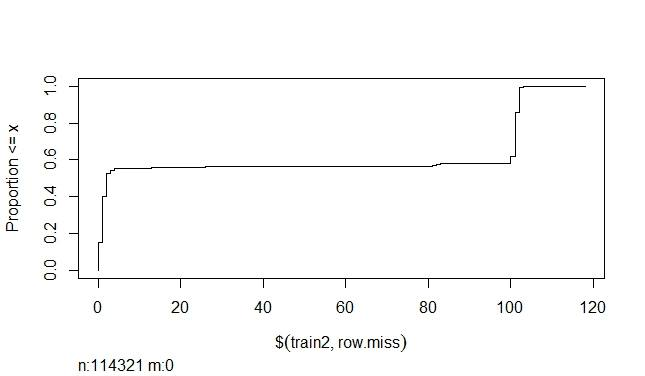
\includegraphics[width=1.0\textwidth]{RowmissEcdf}
\caption{CDF of Missing Values by Rows}

 
\end{figure}
Since there was only about $14\%$ of data with no missing values, the team decided to consider data with only missing values in numeric variables, and then numbers of observed values then increased to around 62,561 observations. By checking the actual data again, we noticed that there was some pattern of missing values across numeric variables: for some observations, values appear to be missing for many of the same numeric variables. Thus we can create new variables based on this information. Figure \ref{f1} is an empirical cumulative distribution function plot which shows missing values calculated by rows. There was a big jump at 0 and another jump at 100. We decided to create 3 variables: 1) count of missing variables, 2) no missing value vs. any missing values, and 3)$<100$ missing values vs $>= 100$ missing values. We then replaced these missing values with mean values because it would have the least impact on models while modeling.
\subsection{Handling Character Variables}
As mentioned in the previous section, some variables were multi-character with length of strings was bigger than one, especially for the variable v22 which has string length more than three. What we did was that we splitted each character within each string and consider them as separate variables (i.e. \enquote{ABCD} => \enquote{A},\enquote{B},\enquote{C},\enquote{D}). The assumption we made here was that, for variables where string length was not fixed, we assumed they were all left-alinged (i.e var = c(\enquote{ABCD}, \enquote{ABC}) => var1 = c(\enquote{A},\enquote{A}); var2= c(\enquote{B},\enquote{B}); var3 = c(\enquote{C},\enquote{C}); var4 = c(\enquote{D},\enquote{ });). Empty values in categorical variables were also considered as a level, and not NA.
Since there were over ten thousands levels in variable v22, and it would be generated too many new variables which might not be useful and affect the computation performance, we then decided to eliminate it from the data. At last, we converted all character variables into dummy variables, with g-1 levels (g = number of levels of unique values of the categorical variable).
\subsection{Near Zero Variables}
After dummy-coding the split character variables, we have 363 variables. However, many of these variables, specifically the dummy variables, may not contain much information due to its \enquote{near zero} property, or having almost constant values across all observations. Such variables can not only give us little to no information, but it may also increase computation time and hinder us from obtaining valuable information from important variables. Thus we will determine and remove \enquote{near zero} variables using the nearZeroVar function in R (from package caret). Using thresholds of maximum frequency ratio (of the most common value to the second most common value in a variable) to 99/1, and a percent unique threshold (percent of number of unique values to total size) to $1\%$. By doing so, we removed 83 variables.


\section{Model design}
Our goal is to find the best model for prediction, namely, identifying whether the claim
can be accelerated. Our candidate models are MLE(Logistic regression), LASSO, ridge, elastic net, SCAD. These methods work in different situations. Suppose the true model is sparse, then LASSO and SCAD may work well. But LASSO tends to drag large value to zero, and may meet problem with correlated variables. SCAD penalty is not convex. Ridge works well in non-sparse model with many predictors with weak effect sizes. Elastic net is a combination of ridge and LASSO, so it has the potential to beat both of them. MLE uses unbiased estimate, since penalized methods increase biases, it still has the chance to beat other methods.  We divided the data into three parts: 
\begin{itemize}
\item Model fitting, selecting tuning parameter.
\item Calculating AUC, selecting threshold. 
\item Calculating error rate.
\end{itemize}

In the first part, we fit models with different tuning parameters and use information criterion to select the best tuning parameter. 
MLE doesn't have tuning parameter, we estimate the coefficients by maximizing the log-likelihood.
LASSO and ridge have one tuning parameter $\lambda$.
Elastic net has two tuning parameters, $\lambda$ and $\alpha$, where $\alpha\in(0,1) $. 
SCAD has two tuning parameters, but set $\alpha=3.7$, which gives good performance in many situations due to simulation (Fan, J. and Li, R., 2001).
We fit a series of models with different tuning parameters and select the best one by information criterion. LASSO and ridge use glmnet default, SCAD use ncvreg default. The series of $\lambda$ is generated like:
$\lambda .min=0.0001\times\lambda .max$. Where $\lambda .max$ is the $\lambda$ such that all coefficients=0. 
Get 100 $\lambda$'s by decreasing from $\lambda .max$ to $\lambda .min$ on a log scale.
Elastic net uses same setting for $\lambda$, but for each $\lambda$, from $alpha$=0.1 to 0.9 fit 9 models (avoids getting the same with LASSO and ridge).  
\\\par
The second part of the data is used for setting threshold. Our goal is to predict 
Our goal is to identify whether a claim can be accelerated, rather than predict a risk.
So that a threshold is needed. After setting a threshold, our predictions can be divided into four categories: true positive, true negative, false positive and false negative.
We need to control  
\begin{equation}
True\ Positive\ Rate=true\ positive/total\ actual\ positive
\end{equation}
\begin{equation}
False\ Negative\ Rate=false\ negative/total\ actual\ negative
\end{equation}
to find the best model.\par
We select the threshold by choosing the point on the curve with the smallest Euclidean distance to (0,1), which stands for the best model in the ROC curve. 

We can also use ROC curve to calculate the area under ROC curve(AUC), which shows the closeness of the model to the ideal one.
\\ \par
Since AUC can just be use to compare the overall performance of models, and we care more about the prediction after selecting the threshold, we use the third part of the data to calculate error rate of the prediction using the best threshold. 

\section{Results and Conclusions}
The final five models we tried are MLE(logistic), Lasso, Ridge, Elastic net and SCAD. As we mentioned above, we divide data into three parts, the first part is used for fitting model and deciding parameters in the model, and the second part of the data is used for calculating the ROC curve which can give us a basic idea of how models work, and we use the final part of data to calculate the error rate for each model. And we compare the error rate to find the best model.
Here are several results we have.
\subsection{Tunning Model Parameters}
When tunning the $\lambda$ in Lasso, Ridge and Elastic net model, we used AIC which is based on the model's prediction performance.
\begin{table}[!ht]
\centering
\caption{Lambda selection}
\label{fig:1}
\begin{tabular}{lll}\hline
method      & Best lambda (based on AIC) & Best lambda (based on BIC) \\\hline
Lasso       & 0.0074                     & 0.0028                     \\
Ridge       & 0.0234                     & 0.0234                     \\
Elastic net & 0.0009                     & 0.0031                  \\\hline  
\end{tabular}
\end{table}
As we can see from the table, the optimal lambda based on both AIC and BIC are pretty small, probably the smallest lambda we tried when fitting the model. Since for train dataset we used, has 'n' 300 times of the 'p', so it is reasonable parameters selection procedure may not works well. 
\subsection{Overall Result}
Although ROC curve can give us an overview of how model works, it can't provide us a exact model to do prediction. So we use ROC curve to calculate the AUC which is the shortest L2 norm distance between point on ROC curve and the optimal point. And use these threshold to calculate error rate for each model method.
\begin{table}[!ht]
\centering
\caption{Result}
\label{fig:1}
\begin{tabular}{llll}
\hline
Model       & AUC   & Threshold for prediction & Error rate \\\hline
MLE         & 0.729 & 0.743                    & 0.339      \\
Lasso       & 0.73  & 0.745                    & 0.34       \\
Ridge       & 0.72  & 0.731                    & 0.342      \\
Elastic Net & 0.73  & 0.745                    & 0.344      \\
SCAD        & 0.732 & 0.746                    & 0.334     \\\hline
\end{tabular}
\end{table}
Comparing these five models, the non-convex model SCAD gives the best performance with highest AUC and smallest 0.334.   \\
It's also interesting that Lasso actual give better AUC than MLE, which implies that regularization works under this situation. 
Deeply looking into the AIC when we choosing  lambda for Lasso and Ridge model, the smallest AIC is reached at the second smallest AIC for lasso model, which means Lasso is doing variable selection.


\begin{thebibliography}{00}
\bibitem[1]{1}Fan, Jianqing, and Runze Li. "Variable selection via nonconcave penalized likelihood and its oracle properties." Journal of the American statistical Association 96.456 (2001): 1348-1360.

\end{thebibliography}


\end{document}



\end{document}